\cleardoublepage
\chapter{Equazioni del campo gravitazionale}
\label{cha:equazioni-campo-grav}

\section{Tensore di Riemann}
\label{sec:tensore-riemann}

\subsection{Definizione e proprietà algebriche}
\label{sec:definizione-proprietà-riemann}

Si può far vedere\footnote{Vedi~\textcite[133-135]{weinberg:gravitation}.} che
l'unico tensore ottenibile dal tensore metrico e dalle sue derivate prime e
seconde è il \emph{tensore di curvatura di Riemann-Christoffel} o,
semplicemente, \index{tensore!di Riemann}\emph{tensore di Riemann}
\begin{equation}
  \tensor{R}{^{\lambda}_{\mu\nu\kappa}}
  = \parder{\tensor{\Gamma}{^{\lambda}_{\mu\nu}}}{x^{\kappa}}
  - \parder{\tensor{\Gamma}{^{\lambda}_{\mu\kappa}}}{x^{\nu}} +
  \tensor{\Gamma}{^{\eta}_{\mu\nu}} \tensor{\Gamma}{^{\lambda}_{\eta\kappa}} -
  \tensor{\Gamma}{^{\eta}_{\mu\kappa}} \tensor{\Gamma}{^{\lambda}_{\eta\nu}}.
\end{equation}
Il tensore di Riemann è un tensore nel senso specificato nel
paragrafo~\ref{sec:tensori}\footnote{Non è immediato riconoscere che
  $\tensor{R}{^{\lambda}_{\mu\nu\kappa}}$ è effettivamente un tensore dato che è
  definito a partire dalla connessione affine, la quale non ha natura
  tensoriale.  Si può trovare una dimostrazione di questa proprietà
  in~\textcite[131-133]{weinberg:gravitation}.}
ed è lineare nelle derivate seconde del tensore metrico.

Per analizzare le proprietà algebriche del tensore di Riemann conviene
considerare la sua forma completamente covariante
\begin{equation}
  \label{eq:riemann-covariante}
  \begin{split}
    R_{\lambda\mu\nu\kappa} &= g_{\lambda\sigma}
    \tensor{R}{^{\sigma}_{\mu\nu\kappa}} = g_{\lambda\sigma}
    \bigg( \parder{\tensor{\Gamma}{^{\lambda}_{\mu\nu}}}{x^{\kappa}}
    - \parder{\tensor{\Gamma}{^{\lambda}_{\mu\kappa}}}{x^{\nu}} +
    \tensor{\Gamma}{^{\eta}_{\mu\nu}} \tensor{\Gamma}{^{\lambda}_{\eta\kappa}} -
    \tensor{\Gamma}{^{\eta}_{\mu\kappa}}
    \tensor{\Gamma}{^{\lambda}_{\eta\nu}} \bigg) \\
    &= \frac{1}{2} \bigg( \parder{g_{\lambda\nu}}{x^{\kappa}, x^{\mu}}
    - \parder{g_{\mu\nu}}{x^{\kappa}, x^{\lambda}}
    - \parder{g_{\lambda\kappa}}{x^{\nu}, x^{\mu}}
    + \parder{g_{\mu\kappa}}{x^{\nu}, x^{\lambda}} \bigg) \\
    &+ g_{\eta\sigma} (\tensor{\Gamma}{^{\eta}_{\nu\lambda}}
    \tensor{\Gamma}{^{\sigma}_{\mu\kappa}} -
    \tensor{\Gamma}{^{\eta}_{\kappa\lambda}}
    \tensor{\Gamma}{^{\sigma}_{\mu\nu}}).
  \end{split}
\end{equation}
Questa relazione ci tornerà utile quando considereremo il limite newtoniano
delle equazioni di Einstein.  Da questa espressione si vede che
\begin{enumerate}
\item \label{item:antisimmetria-riemann} il tensore di Riemann è antisimmetrico
  rispetto allo scambio fra primo e secondo indice e allo scambio fra terzo e
  quarto indice
  \begin{equation}
    R_{\lambda\mu\nu\kappa} = -R_{\mu\lambda\nu\kappa} =
    -R_{\lambda\mu\kappa\nu} = R_{\mu\lambda\kappa\nu};
  \end{equation}
\item \label{item:simmetria-riemann} il tensore di Riemann
  $R_{\lambda\mu\nu\kappa}$ è simmetrico rispetto allo scambio fra la prima
  coppia indici $(\lambda,\mu)$ con la seconda coppia $(\nu,\kappa)$
  \begin{equation}
    R_{\lambda\mu\nu\kappa} = R_{\nu\kappa\lambda\mu};
  \end{equation}
\item \label{item:ciclicita-riemann} è valida la seguente relazione di ciclicità
  (si noti che il primo indice è tenuto fisso, si fanno ruotare gli altri tre)
  \begin{equation}
    \label{eq:ciclicita-riemann}
    R_{\lambda\mu\nu\kappa} + R_{\lambda\kappa\mu\nu} + R_{\lambda\nu\kappa\mu}
    = 0.
  \end{equation}
\end{enumerate}

A causa delle proprietà appena elencate, delle $4^{4} = 256$ componenti del
tensore di Riemann solo $20$ sono indipendenti.  Per far vedere ciò consideriamo
il caso generale di uno spazio $n$-dimensionale.  Il tensore di Riemann può
essere immaginato come una matrice quadrata simmetrica (per la proprietà di
simmetria~\ref{item:simmetria-riemann}) di ordine $d$ del tipo
$R_{(\lambda\mu)(\nu\kappa)}$, con indici $(\lambda\mu)$ e $(\nu\kappa)$.  Il
valore dell'ordine $d$ di questa matrice è dato dal numero di valori
indipendenti che assumono i due indici che, per la proprietà di
antisimmetria~\ref{item:antisimmetria-riemann}, sono uguali al numero di
elementi indipendenti di una matrice $n \times n$ antisimmetrica, cioè
$d = n(n-1)/2$.  Dunque gli elementi indipendenti di
$R_{(\lambda\mu)(\nu\kappa)}$ si riducono
\begin{equation}
  \frac{1}{2} d (d + 1) = \frac{1}{2}\bigg( \frac{1}{2}n(n-1) \bigg) \bigg(
  \frac{1}{2}n(n-1) +1 \bigg) = \frac{1}{8}n(n-1)(n^{2} - n +2).
\end{equation}
% TODO: provare a capire per bene il perché dell'affermazione successiva e a
% spiegarlo in maniera semplice.  Per esempio vedi
% http://www.maths.tcd.ie/~houghton/TEACHING/442/notes/22Oct2002.pdf
% http://sergeysk.wordpress.com/2011/01/21/number-of-independent-components-of-the-riemann-curvature-tensor/
% http://ned.ipac.caltech.edu/level5/March01/Carroll3/Carroll3.html (è il
% capitolo 3 del Carrol)
Infine, la relazione di ciclicità~\eqref{eq:ciclicita-riemann} corrisponde a
$\binom{n}{4}$ equazioni differenti, allora abbiamo altrettanti ulteriori
vincoli, così che gli elementi indipendenti del tensore di Riemann
$n$-dimensionale sono
\begin{equation}
  C_{n} = \frac{1}{8}n(n-1)(n^{2} - n +2) - \binom{n}{4} =
  \frac{1}{12}n^{2}(n^{2} - 1).
\end{equation}
Ponendo $n=4$ abbiamo che nello spazio-tempo quadrimensionale gli elementi
indipendenti del tensore di Riemann sono $C_{4} = 20$, come avevamo
preannunciato.

La contrazione fra primo e terzo indice del tensore di Riemann dà il
\index{tensore!di Ricci}\emph{tensore di Ricci}
\begin{equation}
  \label{eq:tens-ricci}
  R_{\mu\kappa} = g^{\lambda\nu} R_{\lambda\mu\nu\kappa} =
  \tensor{R}{^{\nu}_{\mu\nu\kappa}}
  = \parder{\tensor{\Gamma}{^{\nu}_{\mu\nu}}}{x^{\kappa}}
  - \parder{\tensor{\Gamma}{^{\nu}_{\mu\kappa}}}{x^{\nu}} +
  \tensor{\Gamma}{^{\eta}_{\mu\nu}} \tensor{\Gamma}{^{\nu}_{\eta\kappa}} -
  \tensor{\Gamma}{^{\eta}_{\mu\kappa}} \tensor{\Gamma}{^{\nu}_{\eta\nu}}.
\end{equation}
Il tensore di Ricci è simmetrico per la proprietà~\ref{item:simmetria-riemann}
di simmetria del tensore di Riemann, infatti
\begin{equation}
  \label{eq:simmetria-riemann}
  R_{\mu\kappa} = g^{\lambda\nu} R_{\lambda\mu\nu\kappa} = g^{\lambda\nu}
  R_{\nu\kappa\lambda\mu} = g^{\nu\lambda} R_{\nu\kappa\lambda\mu} =
  R_{\kappa\mu}.
\end{equation}
Dunque delle $4^{2} = 16$ componenti del tensore solo $10$ sono indipendenti.
Inoltre il tensore di Ricci è essenzialmente l'unico tensore non nullo che si
può ottenere dalla contrazione del tensore di Riemann.  Contraendo primo e
secondo indice, per la proprietà~\ref{item:antisimmetria-riemann} di
antisimmetria del tensore di Riemann si ha
\begin{equation}
  \tensor{R}{^{\mu}_{\mu\nu\kappa}} = g^{\lambda\mu}
  R_{\lambda\mu\nu\kappa} = -g^{\lambda\mu} R_{\mu\lambda\nu\kappa} =
  -g^{\mu\lambda}R_{\mu\lambda\nu\kappa} =
  -g^{\lambda\mu}R_{\lambda\mu\nu\kappa} = 0.
\end{equation}
Analogamente, contraendo terzo e quarto indice si ottiene
\begin{equation}
  \tensor{R}{_{\lambda\mu}^{\kappa}_{\kappa}} = g^{\nu\kappa}
  R_{\lambda\mu\nu\kappa} = 0.
\end{equation}
Contraendo secondo e quarto indice del tensore di Riemann si ottiene di nuovo il
tensore di Ricci, invece contraendo primo e quarto indice oppure secondo terzo
si ottiene ancora il tensore di Ricci così come da noi definito ma con il segno
opposto.  Infatti, moltiplicando tutti i membri
della~\eqref{eq:simmetria-riemann} per $g^{\lambda\nu}$ troviamo
\begin{equation}
  \tensor{R}{^{\nu}_{\mu\nu\kappa}} = -\tensor{R}{_{\mu}^{\nu}_{\nu\kappa}} =
  -\tensor{R}{^{\nu}_{\mu\kappa\nu}} = \tensor{R}{_{\mu}^{\nu}_{\kappa\nu}}.
\end{equation}

L'ulteriore contrazione del tensore di Ricci dà la
\index{curvatura scalare}\emph{curvatura scalare}
\begin{equation}
  R = g^{\mu\nu}R_{\mu\nu} = \tensor{R}{^{\mu}_{\mu}}.
\end{equation}

\subsection{Tensore di Riemann e curvatura dello spazio}
\label{sec:riemann-curvatura}

Anche in uno spazio piatto è possibile introdurre una metrica non costante su
tutto lo spazio che faccia apparire lo spazio curvo, come se ci fosse un campo
gravitazionale.  Questo è il caso, per esempio, delle coordinate sferiche o
cilindriche nello spazio cartesiano $\R^{3}$.  Siamo allora interessati a
cercare uno strumento che ci permetta di discriminare fra uno spazio-tempo
intrinsecamente curvo, perché permeato da un reale campo gravitazionale, e uno
spazio-tempo piatto, cioè lo spazio di Minkowski, in cui si fa uso di coordinate
curvilinee.  Se siamo nella seconda situazione, in questo spazio di Minkowski è
possibile effettuare una trasformazione delle coordinate
$x^{\alpha} \to \xi^{\alpha}(x)$ da un sistema di coordinate curvilinee
$x^{\alpha}$ con tensore metrico $g_{\mu\nu}$ non costante a un sistema di
coordinate $\xi^{\alpha}(x)$ con tensore metrico uguale al tensore di Minkowski
$\eta_{\alpha\beta}$ e in tutto lo spazio si ha
\begin{equation}
  \eta_{\alpha\beta} =
  g_{\mu\nu} \parder{x^{\mu}}{\xi^{\alpha}} \parder{x^{\nu}}{\xi^{\beta}}.
\end{equation}
Per il \index{principio!di equivalenza}principio di equivalenza, in ogni punto
$X$ dello spazio è possibile individuare un sistema di coordinate localmente
inerziali $\xi_{X}$ che soddisfano la relazione precedente in un intorno
infinitesimo di $X$.  Noi invece vogliamo scoprire se esista un sistema di
coordinate $\xi^{\alpha}$ che soddisfi la relazione in tutto lo spazio.

Lo strumento a cui siamo interessati è il tensore di Riemann, infatti è
possibile dimostrare\footnote{Vedi~\textcite[138]{weinberg:gravitation}.} il
seguente
\begin{teorema}
  Condizioni necessarie e sufficienti affinché sia possibile effettuare una
  trasformazione di coordinate $x \to \xi$ tale che in tutto lo spazio sia
  valida la relazione
  \begin{equation}
    \label{eq:tensore-spazio-piatto}
    \eta_{\alpha\beta} =
    g_{\mu\nu} \parder{x^{\mu}}{\xi^{\alpha}} \parder{x^{\nu}}{\xi^{\beta}}
  \end{equation}
  sono
  \begin{enumerate}
  \item il \index{tensore!di Riemann}tensore di Riemann si annulla in tutto lo
    spazio
    \begin{equation}
      \tensor{R}{^{\lambda}_{\mu\nu\kappa}} = 0;
    \end{equation}
  \item in qualche punto $X$ la matrice $g_{\mu\nu}(X)$ ha tre autovalori
    positivi e uno negativo.
  \end{enumerate}
\end{teorema}
Il fatto che sia valida la relazione~\eqref{eq:tensore-spazio-piatto} significa
che la metrica è quella usuale dello spazio di Minkowski
$\dd \tau^{2} = \dd t^{2} - \dd\bm{x}^{2}$, l'annullarsi del tensore di Riemann
invece significa che la curvatura dello spazio è nulla, il teorema precedente
dichiara l'equivalenza fra queste due condizioni.  In questo modo il tensore di
Riemann ci permette di verificare se nello spazio sia presente un reale campo
gravitazionale.

Un altro modo che permette di mostrare che il tensore di Riemann caratterizza la
curvatura dello spazio, e quindi evidenzia la presenza di un campo
gravitazionale, è il seguente.  Dato un vettore covariante $V_{\mu}$ si dimostra
(vedi l'appendice~\ref{sec:dimostr-derivate-miste-vettore}) che le sue derivate
covarianti seconde miste non commutano
\begin{equation}
  \label{eq:derivate-miste-vettore}
  V_{\mu;\nu;\kappa} - V_{\mu;\kappa;\nu} = -V_{\lambda}
  \tensor{R}{^{\lambda}_{\mu\nu\kappa}}.
\end{equation}
Si trovano inoltre analoghe relazioni per i vettori controvarianti o, più in
generale, per i tensori
\begin{subequations}
  \begin{gather}
    \tensor{V}{^{\mu}_{;\nu;\kappa}} - \tensor{V}{^{\mu}_{;\kappa;\nu}} =
    V^{\sigma} \tensor{R}{^{\lambda}_{\sigma\nu\kappa}}, \\
    \tensor{T}{^{\lambda}_{\mu;\nu;\kappa}} -
    \tensor{T}{^{\lambda}_{\mu;\kappa;\nu}} = \tensor{T}{^{\sigma}_{\mu}}
    \tensor{R}{^{\lambda}_{\sigma\nu\kappa}} - \tensor{T}{^{\lambda}_{\sigma}}
    \tensor{R}{^{\sigma}_{\mu\nu\kappa}}.
  \end{gather}
\end{subequations}
Nello spazio di Minkowski le derivate covarianti coincidono con le derivate
ordinarie e le derivate seconde miste commutano
\begin{equation}
  V_{\mu,\nu,\kappa} = \parder{V_{\mu}}{x^{\nu}, x^{\kappa}}
  = \parder{V_{\mu}}{x^{\kappa}, x^{\nu}} = V_{\mu,\kappa,\nu}
\end{equation}
e questo è possibile solo se il tensore di Riemann è identicamente nullo in
tutto lo spazio.

\subsection{Identità di Bianchi}
\label{sec:identita-bianchi}

Si dimostra (vedi l'appendice~\ref{sec:dimostr-identita-bianchi}) la seguente
relazione
\begin{equation}
  \label{eq:bianchi}
  R_{\lambda\mu\nu\kappa;\eta} + R_{\lambda\mu\kappa\eta;\nu} +
  R_{\lambda\mu\eta\nu;\kappa} = 0
\end{equation}
chiamata \index{identità!di Bianchi}\emph{identità di Bianchi}.  Contraiamo gli
indici $\lambda$ e $\nu$ moltiplicando ambo i membri per $g^{\lambda\nu}$
\begin{equation}
  \begin{split}
    \tensor{R}{^{\nu}_{\mu\nu\kappa;\eta}} +
      \tensor{R}{^{\nu}_{\mu\kappa\eta;\nu}} +
    \tensor{R}{^{\nu}_{\mu\eta\nu;\kappa}} &= R_{\mu\kappa;\eta} +
    \tensor{R}{^{\nu}_{\mu\kappa\eta;\nu}} - R_{\mu\eta;\kappa} \\
    &= R_{\mu\kappa;\eta} - \tensor{R}{^{\nu}_{\mu\eta\kappa;\nu}} -
    R_{\mu\eta;\kappa} = 0.
  \end{split}
\end{equation}
Abbiamo sfruttato il fatto che innalzamento degli indici e derivazione
covariante commutano.  Contraendo ulteriormente gli indici $\mu$ e $\kappa$,
cioè moltiplicando gli ultimi due membri per $g^{\mu\kappa}$, otteniamo
\begin{equation}
  R_{;\eta} - \tensor{R}{^{\nu}_{\eta;\nu}} -
  \tensor{R}{^{\kappa}_{\eta;\kappa}} = R_{;\eta} - 2
  \tensor{R}{^{\mu}_{\eta;\mu}} = 0,
\end{equation}
poiché $\kappa$ e $\nu$ sono entrambi indici muti che abbiamo rinominato $\mu$.
Questa relazione può anche essere scritta come
\begin{equation}
  \bigg( \tensor{R}{^{\mu}_{\eta}} - \frac{1}{2} \tensor{\delta}{^{\mu}_{\eta}}
  R \bigg)_{;\mu} = 0
\end{equation}
e moltiplicando ancora per $g^{\eta\nu}$
\begin{equation}
  \bigg( R^{\mu\nu} - \frac{1}{2} g^{\mu\nu} R\bigg)_{;\mu} = 0.
\end{equation}
La quantità all'interno delle parentesi è il
\index{tensore!di Einstein}\emph{tensore di Einstein}
\begin{equation}
  G^{\mu\nu} = R^{\mu\nu} - \frac{1}{2} g^{\mu\nu}R
\end{equation}
e abbiamo dunque mostrato che ha quadridivergenza covariante nulla
\begin{equation}
  \label{eq:divergenza-tens-einstein}
  \tensor{G}{^{\mu\nu}_{;\mu}} = \bigg( R^{\mu\nu} - \frac{1}{2} g^{\mu\nu}
  R\bigg)_{;\mu} = 0.
\end{equation}

% TODO: scrivere qualcosa.  Vedi lezioni dei giorni 03-04/05/2012
\subsection{\completare{Equazione di deviazione geodetica}}
\label{sec:deviazione-geodetica}

\section{Equazioni di Einstein}
\label{sec:equazioni-einstein}

\emph{Nota: in questo paragrafo indicheremo esplicitamente la velocità della
  luce nel vuoto $c$.}

Vogliamo ora determinare le equazioni del campo gravitazionale $g_{\mu\nu}$ a
partire dal principio variazionale di Hamilton.  Assumiamo che l'azione $S$ sia
somma di una componente $S_{\textup{g}}$ che descrive solo il campo
gravitazionale e una componente $S_{\textup{m}}$ relativa alla materia che
interagisce con il campo.  L'azione deve essere uno scalare, in modo che risulti
invariante per trasformazioni arbitrarie delle coordinate, e dipenderà dal
tensore metrico, dalle sue derivate prime, dalle coordinate generalizzate $q$ e
dalle velocità generalizzate $\lparder{q}{x^{\lambda}}$,
$S = S(g_{\mu\nu}, \lparder{g_{\mu\nu}}{x^{\lambda}}; q,
\lparder{q}{x^{\lambda}})$.
Hilbert propose questa espressione per l'azione del campo
gravitazionale\footnote{Il fattore davanti all'integrale è stato scelto in
  maniera tale che nel limite newtoniano si ottenga l'equazione di Poisson
  $\nabla^{2} \phi = 4\pi G\rho$.}
\begin{equation}
  S_{\textup{g}} = -\frac{c^{3}}{16\pi G} \int R \sqrt{g} \dd^{4} x,
\end{equation}
chiamata \index{azione!di Hilbert-Einstein} \emph{azione di Hilbert-Einstein}.
$G = \SI{6.673 84(80)e-11}{\cubic\metre\per\kilo\metre\per\second\squared}$ è la
\index{costante!di gravitazione universale}
\emph{costante di gravitazione universale}.  L'azione della materia ha invece
espressione\footnote{In uno spazio-tempo piatto $g = 1$, quindi
  $S_{\textup{m}} = (1/c)\int \Lambda \dd^{4} x = \iint \Lambda \dd t\dd^{3}
  \bm{x}$, come nella~\eqref{eq:azione-campo}.}
\begin{equation}
  S_{\textup{m}} = \frac{1}{c} \int \Lambda \sqrt{g} \dd^{4} x,
\end{equation}
in cui $\Lambda = \Lambda(g^{\mu\nu}, \partial_{\lambda}g^{\mu\nu})$ è la densità
di lagrangiana associata al sistema che interagisce con il campo
gravitazionale.  L'interazione fra il campo e la materia è inclusa in
$S_{\textup{m}}$.

Per determinare le equazioni del campo gravitazionale dobbiamo richiedere che
l'azione sia stazionaria rispetto alle variazioni, a volume fissato,
$\delta g_{\mu\nu}$ del campo che devono soddisfare inoltre la condizione che si
annullino sul bordo dell'ipervolume di integrazione.  Dunque dobbiamo imporre
$\delta S = \delta(S_{\textup{g}} + S_{\textup{m}}) = 0$.  Calcoliamo il
contributo di $\delta S_{\textup{g}}$
\begin{equation}
  \label{eq:var-HE}
  \begin{split}
    \delta \int R \sqrt{g} \dd^{4} x &= \delta \int g^{\mu\nu} R_{\mu\nu}
    \sqrt{g} \dd^{4} x \\
    &= \int (\delta g^{\mu\nu} R_{\mu\nu} \sqrt{g} + g^{\mu\nu} R_{\mu\nu}
    \delta \sqrt{g} + g^{\mu\nu} \delta R_{\mu\nu} \sqrt{g}) \dd^{4} x.
  \end{split}
\end{equation}
Osserviamo che
\begin{equation}
  \delta\sqrt{g} = \parder{\sqrt{g}}{g} \parder{g}{g^{\mu\nu}} \delta g^{\mu\nu}
  = \frac{1}{2 \sqrt{g}} (-g g_{\mu\nu} ) \delta g^{\mu\nu} = - \frac{1}{2}
  g_{\mu\nu} \sqrt{g} \delta g^{\mu\nu},
\end{equation}
in cui abbiamo ricordato la~\eqref{eq:g_mu_rho-determinante2}.  Sostituendo
nella~\eqref{eq:var-HE} otteniamo
\begin{equation}
  \delta \int R \sqrt{g} \dd^{4} x = \int \bigg( R_{\mu\nu} - \frac{1}{2}
  g_{\mu\nu} R \bigg)\sqrt{g} \delta g^{\mu\nu} \dd^{4} x + \int g^{\mu\nu}
  \delta R_{\mu\nu} \sqrt{g} \dd^{4} x.
\end{equation}
Mostriamo che il secondo integrale è nullo.  Innanzitutto la
\index{tensore!di Ricci!variazione del}variazione del tensore di Ricci può
essere espressa in termini di variazioni della connessione affine mediante
l'\index{identità!di Palatini}% TODO: vedere di dimostrarla
\emph{identità di
  Palatini}\footnote{Si
  noti che la variazione della connessione affine è un tensore poiché è la
  differenza fra due connessioni affini, la quale è un tensore come visto nel
  paragrafo~\ref{sec:connessione-affine}.}
\begin{equation}
  \delta R_{\mu\nu} = (\delta \tensor{\Gamma}{^{\lambda}_{\mu\lambda}})_{;\nu} -
  (\delta \tensor{\Gamma}{^{\lambda}_{\mu\nu}})_{;\lambda}.
\end{equation}
Allora si può riscrivere l'integrale in esame come
\begin{equation}
  \int g^{\mu\nu} \delta R_{\mu\nu} \sqrt{g} \dd^{4} x = \int (g^{\mu\nu} \delta
  \tensor{\Gamma}{^{\lambda}_{\mu\lambda;\nu}} - g^{\mu\nu} \delta
  \tensor{\Gamma}{^{\lambda}_{\mu\nu;\lambda}}) \sqrt{g} \dd^{4} x
\end{equation}
e per il teorema di Gauss in forma covariante~\eqref{eq:gauss-covariante}
ricaviamo
\begin{equation}
  \begin{split}
    \int g^{\mu\nu} \delta R_{\mu\nu} \sqrt{g} \dd^{4} x &= \int (\delta
    \tensor{\Gamma}{^{\lambda\nu}_{\lambda;\nu}} - \delta
    \tensor{\Gamma}{^{\lambda\nu}_{\nu;\lambda}}) \sqrt{g} \dd^{4} x \\
    &= \int \delta \tensor{\Gamma}{^{\lambda\nu}_{\lambda}} \sqrt{g} \dd
    \Sigma_{\nu} - \int \delta \tensor{\Gamma}{^{\lambda\nu}_{\lambda}} \sqrt{g}
    \dd \Sigma_{\lambda} = 0
  \end{split}
\end{equation}
poiché gli integrali sulle ipersuperfici vanno calcolati sul bordo
dell'ipervolume costante su cui si calcola la variazione dell'azione e sul bordo
sono nulle le variazioni di $g_{\mu\nu}$ e quindi anche della connessione
affine, la quale dipende dal tensore metrico.  Dunque abbiamo trovato che la
variazione dell'azione di Hilbert-Einstein è
\begin{equation}
  \delta S_{\textup{g}} = -\frac{c^{3}}{16\pi G} \int \bigg( R_{\mu\nu} -
  \frac{1}{2} g_{\mu\nu} R \bigg)\sqrt{g} \delta g^{\mu\nu} \dd^{4} x.
\end{equation}

Per calcolare la variazione $\delta S_{\textup{m}}$ dell'azione associata alla
materia ragioniamo in maniera analoga a quanto fatto nel
paragrafo~\ref{sec:tensore-energia-impulso}
\begin{equation}
  \begin{split}
    \delta S_{\textup{m}} &= \frac{1}{c} \delta \int \Lambda(g^{\mu\nu},
    \tensor{g}{^{\mu\nu}_{,\lambda}}) \sqrt{g} \dd^{4} x = \frac{1}{c} \int
    \bigg( \parder{(\sqrt{g}\Lambda)}{g^{\mu\nu}} \delta g^{\mu\nu}
    + \parder{(\sqrt{g}\Lambda)}{\tensor{g}{^{\mu\nu}_{,\lambda}}}
    \delta \tensor{g}{^{\mu\nu}_{,\lambda}} \bigg) \dd^{4} x \\
    &= \frac{1}{c} \int \bigg( \parder{(\sqrt{g}\Lambda)}{g^{\mu\nu}} \delta
    g^{\mu\nu} + \parder{}{x^{\lambda}}
    \bigg( \parder{(\sqrt{g}\Lambda)}{\tensor{g}{^{\mu\nu}_{,\lambda}}} \delta
    g^{\mu\nu}\bigg) - \delta g^{\mu\nu} \parder{}{x^{\lambda}}
    \bigg( \parder{(\sqrt{g}\Lambda)}{\tensor{g}{^{\mu\nu}_{,\lambda}}} \bigg)
    \bigg) \dd^{4} x \\
    &= \frac{1}{c} \int \bigg( \parder{(\sqrt{g}\Lambda)}{g^{\mu\nu}}
    - \parder{}{x^{\lambda}}
    \bigg( \parder{(\sqrt{g}\Lambda)}{\tensor{g}{^{\mu\nu}_{,\lambda}}} \bigg)
    \bigg) \delta g^{\mu\nu} \dd^{4} x.
  \end{split}
\end{equation}
Nell'ultimo passaggio abbiamo sfruttato il fatto che l'integrale del secondo
termine si trasforma, per il teorema di Gauss, in un integrale sul bordo del
volume di integrazione sul quale le variazioni $\delta g^{\mu\nu}$ sono nulle.
Introduciamo il tensore $T_{\mu\nu}$ definito
da\footnote{Si noti che \textcites{barone:relativita,landau:campi} definisco
  questo tensore con il segno opposto a causa della diversa convenzione sui
  segni.  Vedi pagina~\pageref{eq:convenzione-segni}.}
\begin{equation}
  -\frac{1}{2} \sqrt{g} T_{\mu\nu} = \parder{(\sqrt{g}\Lambda)}{g^{\mu\nu}}
  - \parder{}{x^{\lambda}}
  \bigg( \parder{(\sqrt{g}\Lambda)}{\tensor{g}{^{\mu\nu}_{,\lambda}}} \bigg)
\end{equation}
% TODO: spiegare da qualche parte che questo è proprio il tensore
% energia-impulso (e mettere \index{tensore!energia-impulso})
così la variazione dell'azione della materia diventa
\begin{equation}
  \delta S_{\textup{m}} = -\frac{1}{2c} \int T_{\mu\nu} \delta g^{\mu\nu}
  \sqrt{g} \dd^{4} x
\end{equation}
e la condizione di stazionarietà dell'azione totale del sistema campo
gravitazionale + particelle interagenti è
\begin{equation}
  \delta S = \delta(S_{\textup{g}} + S_{\textup{m}}) = -\int \bigg(
  \frac{c^{3}}{16\pi G} \bigg( R_{\mu\nu} - \frac{1}{2} g_{\mu\nu} R \bigg) +
  \frac{1}{2c} T_{\mu\nu} \bigg) \sqrt{g} \delta g^{\mu\nu} \dd^{4} x = 0.
\end{equation}
Data l'arbitrarietà delle variazioni $\delta g^{\mu\nu}$ ricaviamo
\begin{equation}
  \label{eq:einstein}
  G_{\mu\nu} = R_{\mu\nu} - \frac{1}{2} g_{\mu\nu} R = -\frac{8\pi G}{c^{4}}
  T_{\mu\nu}
\end{equation}
che sono le \emph{equazioni del campo gravitazionale} in presenza di sorgenti,
chiamate anche \index{equazioni!di Einstein}\emph{equazioni di Einstein}.
Osserviamo che dalla~\eqref{eq:divergenza-tens-einstein} deriva che anche il
tensore energia-impulso della materia ha quadridivergenza covariante nulla
$\tensor{T}{^{\mu\nu}_{;\mu}} = 0$.

Moltiplicando gli ultimi due membri per $g^{\mu\nu}$, in modo da contrarre gli
indici $\mu$ e $\nu$, otteniamo
\begin{equation}
  R - \frac{1}{2}4R = -R = -\frac{8\pi G}{c^{4}}\tensor{T}{^{\lambda}_{\lambda}}
\end{equation}
e sostituendo nella~\eqref{eq:einstein} otteniamo un'espressione alternativa per
le \index{equazioni!di Einstein}equazioni di Einstein
\begin{equation}
  R_{\mu\nu} = -\frac{8\pi G}{c^{4}} \bigg( T_{\mu\nu} -
  \frac{1}{2}g_{\mu\nu}\tensor{T}{^{\lambda}_{\lambda}} \bigg).
\end{equation}
Da qui possiamo osservare che nel vuoto, cioè in assenza di materia, il tensore
energia-impulso è nullo quindi le \index{equazioni!di Einstein}equazioni di
Einstein si riducono a
\begin{equation}
  R_{\mu\nu} = 0.
\end{equation}
Si noti che questa equazione non significa che uno spazio-tempo vuoto è anche
piatto, per avere quest'ultima condizione deve verificarsi la condizione più
forte $\tensor{R}{^{\lambda}_{\mu\nu\kappa}} = 0$.

\subsection{Limite newtoniano delle equazioni di Einstein}
\label{sec:limite-newtoniano-einstein}

Vogliamo determinare il limite newtoniano (campi gravitazionali deboli e
statici, velocità non relativistiche) delle equazioni di Einstein e per fare
questo lavoriamo in maniera analoga a quanto fatto nel
paragrafo~\ref{sec:limite-newtoniano}, quindi poniamo
$g_{\mu\nu} = \eta_{\mu\nu} + h_{\mu\nu}$.  Ci aspettiamo che il tensore
energia-impulso sia in queste condizioni quello ricavato nel limite di basse
velocità nel paragrafo~\ref{sec:fluido-perfetto} per un corpo macroscopico
continuo (come un \index{fluido!perfetto}fluido perfetto)
\begin{subequations}
  \begin{align}
    T_{ij} &= \rho c^{2} u_{i} u_{j}, \\
    T_{00} &= \rho c^{2},
  \end{align}
\end{subequations}
in cui qui con $\rho$ indichiamo la densità di massa a riposo (e quindi
$\rho c^{2}$ è la densità di energia a riposo, per brevità omettiamo il pedice
$0$) e $u_{\mu}$ la quadrivelocità.  Per l'ipotesi di velocità non
relativistiche si devono trascurare le componenti spaziali della quadrivelocità
rispetto alla componente temporale, cioè $u_{i} = 0$, e quindi $T_{ij} = 0$ da
cui abbiamo inoltre
\begin{equation}
  0 = G_{ij} \approx R_{ij} - \frac{1}{2}\eta_{ij}R.
\end{equation}
Allora l'unica equazione di Einstein rilevante è quella con $G_{00}$.
Contraendo gli indici dell'equazione precedente otteniamo
\begin{equation}
  \eta^{ij}R_{ij} \approx \frac{1}{2} \eta_{ij}\eta^{ij} R = \frac{3}{2} R.
\end{equation}
La curvatura scalare può essere approssimata come
\begin{equation}
  R = g^{\mu\nu}R_{\mu\nu} \approx \eta^{\mu\nu} R_{\mu\nu} = \eta^{00}R_{00} +
  \eta^{ij}R_{ij} = -R_{00} + \frac{3}{2} R
\end{equation}
dunque $R \approx 2 R_{00}$.  Sostituendo nell'equazione di Einstein abbiamo
\begin{equation}
  G_{00} = R_{00} - \frac{1}{2} \eta_{00}R = R_{00} + \frac{1}{2} R = 2 R_{00} =
  -\frac{8\pi G}{c^{4}} T_{00} = -\frac{8\pi G}{c^{4}} \rho c^{2}
\end{equation}
da cui
\begin{equation}
  R_{00} = -\frac{4\pi G}{c^{2}} \rho.
\end{equation}
D'altra parte osserviamo che
\begin{equation}
  R_{00} = g^{\mu\nu}R_{\mu 0\nu 0} \approx \eta^{\mu\nu}R_{\mu 0\nu 0}
\end{equation}
Dalla~\eqref{eq:riemann-covariante}, arrestandoci ai termini del primo ordine in
$h_{\mu\nu}$, abbiamo
\begin{equation}
  \label{eq:riemann-approx}
  \begin{split}
    R_{\lambda\mu\nu\kappa} &\approx \frac{1}{2}
    \bigg( \parder{h_{\lambda\nu}}{x^{\kappa}, x^{\mu}}
    - \parder{h_{\mu\nu}}{x^{\kappa},
      x^{\lambda}}- \parder{h_{\lambda\kappa}}{x^{\nu}, x^{\mu}}
    + \parder{h_{\mu\kappa}}{x^{\nu}, x^{\lambda}} \bigg) \\
    &+ \eta_{\eta\sigma}
    (\underbrace{\tensor{\Gamma}{^{\eta}_{\nu\lambda}}
      \tensor{\Gamma}{^{\sigma}_{\mu\kappa}} -
      \tensor{\Gamma}{^{\eta}_{\kappa\lambda}}
      \tensor{\Gamma}{^{\sigma}_{\mu\nu}}}_{\mathcal{O}(h^{2})}) \\
    &= \frac{1}{2} \bigg( \parder{h_{\lambda\nu}}{x^{\kappa}, x^{\mu}}
    - \parder{h_{\mu\nu}}{x^{\kappa},
      x^{\lambda}}- \parder{h_{\lambda\kappa}}{x^{\nu}, x^{\mu}}
    + \parder{h_{\mu\kappa}}{x^{\nu}, x^{\lambda}} \bigg) + \mathcal{O}(h^{2})
  \end{split}
\end{equation}
e in particolare, sfruttando l'ipotesi di campi costanti,
\begin{subequations}
  \begin{align}
    R_{0000} &\approx 0, \\
    R_{i0j0} &\approx \frac{1}{2} \parder{h_{00}}{x^{i},x^{j}}
  \end{align}
\end{subequations}
allora
\begin{equation}
  R_{00} = \eta^{00}R_{0000} + \eta^{ij}R_{i0j0} = \delta^{ij}R_{i0j0} \approx
  \frac{1}{2}\nabla^{2} h_{00} = -\nabla^{2}\frac{\phi}{c^{2}}
\end{equation}
avendo ricordato la~\eqref{eq:h00}.  Dunque mettendo insieme le due espressioni
di $R_{00}$ ottenute troviamo
\index{equazione!di Poisson!per il campo gravitazionale}l'equazione di Poisson
per il campo gravitazionale
\begin{equation}
  \nabla^{2} \phi = 4\pi G\rho.
\end{equation}

\section{Campo gravitazionale statico e a simmetria sferica}
\label{sec:campo-statico-sferico}

Vogliamo determinare la metrica per un campo gravitazionale a simmetria sferica
e statico, cioè tale che $\dd\tau^{2} = -g_{\mu\nu}\dd x^{\mu}\dd x^{\nu}$ non
dipenda dalla coordinata temporale $x^{0}$ e dipenda dalle coordinate spaziali
solo attraverso delle quantità invarianti per rotazioni, cioè
$\bm{x} \cdot \dd\bm{x}$, $\bm{x} \cdot \bm{x}$, $\dd\bm{x} \cdot \dd\bm{x}$.
La forma più generale per una metrica con queste proprietà è
\begin{equation}
  \dd\tau^{2} = F(r) \dd t^{2} - 2E(r) \bm{x} \cdot \dd\bm{x} \dd t -
  D(r)(\bm{x} \cdot \dd\bm{x})^{2} - C(r)\dd\bm{x}^{2},
\end{equation}
in cui $F$, $E$, $D$ e $C$ sono funzioni della distanza dall'origine del campo
gravitazionale $r = \norm{\bm{x}}$.  Data la simmetria del sistema che vogliamo
analizzare conviene passare in coordinate sferiche
\begin{subequations}
  \begin{align}
    x^{1} &= r \sin\theta \cos\phi, \\
    x^{2} &= r \sin\theta \sin\phi, \\
    x^{3} &= r \cos\theta
  \end{align}
\end{subequations}
così che la metrica diventa
\begin{equation}
  \dd\tau^{2} = F(r) \dd t^{2} - 2E(r) r\dd r\dd t - r^{2}D(r)\dd r^{2} -
  C(r)(\dd r^{2} + r^{2}\dd\theta^{2} + r^{2}\sin^{2}\theta \dd\phi^{2}).
\end{equation}
La libertà che si ha, in relatività generale, nella scelta del sistema di
coordinate ci consente di semplificare questa espressione.  Consideriamo dunque
la trasformazione della coordinate temporale $t \to t' = t + \phi(r)$ con la
condizione
\begin{equation}
  \toder{\phi}{r} = - r\frac{E(r)}{F(r)}
\end{equation}
in modo da annullare il termine $g_{rt}$ del tensore metrico.  Così la metrica
diventa
\begin{equation}
  \dd \tau^{2} = F(r)\dd t'^{2} - G(r)\dd r^{2} -C(r)(\dd r^{2} +
  r^{2}\dd\theta^{2} + r^{2}\sin^{2}\theta \dd\phi^{2})
\end{equation}
con
\begin{equation}
  G(r) = r^{2} \bigg(D(r) + \frac{E^{2}(r)}{F(r)} \bigg).
\end{equation}
Effettuando inoltre la trasformazione $r \to r' = C(r)r^{2}$ otteniamo la
\index{metrica!forma standard della}\emph{forma standard} della metrica
(rinominiamo le variabili $r'$ e $t'$ in $r$ e $t$)
\begin{equation}
  \label{eq:metrica-standard}
  \dd\tau^{2} = B(r)\dd t^{2} - A(r)\dd r^{2} - r^{2}(\dd\theta^{2} +
  \sin^{2}\theta \dd\phi^{2}),
\end{equation}
in cui
\begin{subequations}
  \begin{align}
    B(r) &= F(r), \\
    A(r) &= \bigg(1 + \frac{G(r)}{C(r)} \bigg) \bigg( 1 + \frac{r}{2C(r)}
    \toder{C(r)}{r} \bigg)^{-2}.
  \end{align}
\end{subequations}
Il tensore metrico è rappresentato dalla seguente matrice diagonale
\begin{equation}
  g_{\mu\nu} =
  \begin{pmatrix}
    g_{tt}       & g_{tr}       & g_{t\theta}      & g_{t\phi}      \\
    g_{rt}       & g_{rr}       & g_{r\theta}      & g_{r\phi}      \\
    g_{\theta t} & g_{\theta r} & g_{\theta\theta} & g_{\theta\phi} \\
    g_{\phi t}   & g_{\phi r}   & g_{\phi\theta}   & g_{\phi\phi}
  \end{pmatrix}
  =
  \begin{pmatrix}
    -B(r) & 0    & 0     & 0 \\
    0     & A(r) & 0     & 0 \\
    0     & 0    & r^{2} & 0 \\
    0     & 0    & 0     & r^{2}\sin^{2}\theta
  \end{pmatrix}.
\end{equation}
Poiché $g_{\mu\nu}$ è diagonale, gli elementi del tensore metrico controvariante
sono semplicemente $g^{\mu\nu} = 1/g_{\mu\nu}$, quindi
$g^{\mu\nu} = \diag(-B^{-1}(r), A^{-1}(r), r^{-2}, r^{-2}\sin^{-2}\theta)$.
Osserviamo che $g = -\det(g_{\mu\nu}) = r^{4}A(r)B(r)\sin^{2}\theta$, quindi
l'elemento di volume invariante è
\begin{equation}
  \sqrt{-g} \dd^{4} x = r^{2}\sqrt{A(r) B(r)} \sin\theta \dd^{4} x.
\end{equation}

Le connessioni affini possono essere calcolate con la
formula~\eqref{eq:connessione-metrica}.  Si trova che le uniche componenti non
nulle sono
\begin{subequations}
  \begin{align}
    \tensor{\Gamma}{^{r}_{rr}} &= \frac{A'(r)}{2A(r)}, &
    \tensor{\Gamma}{^{r}_{\theta\theta}} &= -\frac{r}{A(r)}, &
    \tensor{\Gamma}{^{r}_{\phi\phi}} &= -\frac{r \sin^{2}\theta}{A(r)}, \\
    \tensor{\Gamma}{^{r}_{tt}} &= \frac{B'(r)}{2A(r)}, &
    \tensor{\Gamma}{^{\theta}_{r\theta}} &=
    \tensor{\Gamma}{^{\theta}_{\theta r}} = \frac{1}{r}, &
    \tensor{\Gamma}{^{\theta}_{\phi\phi}} &= -\sin\theta \cos\theta, \\
    \tensor{\Gamma}{^{\phi}_{\phi r}} &= \tensor{\Gamma}{^{\phi}_{r\phi}} =
    \frac{1}{r}, & \tensor{\Gamma}{^{\phi}_{\phi\theta}} &=
    \tensor{\Gamma}{^{\phi}_{\theta\phi}} = \cot\theta, &
    \tensor{\Gamma}{^{t}_{tr}} &= \tensor{\Gamma}{^{t}_{rt}} =
    \frac{B'(r)}{2B(r)}.
  \end{align}
\end{subequations}
L'apice indica la derivazione rispetto a $r$.

Dopo di ciò è possibile calcolare il tensore di Ricci usando la sua
definizione~\eqref{eq:tens-ricci}.  Grazie all'invarianza per rotazioni e
l'indipendenza dal tempo della metrica, anche il tensore di Ricci è diagonale
con componenti non nulle
\begin{subequations}
  \label{eq:ricci-sferico}
  \begin{align}
    R_{tt} &= -\frac{B''(r)}{2A(r)} + \frac{1}{4} \frac{B'(r)}{A(r)}
    \bigg(\frac{A'(r)}{A(r)} + \frac{B'(r)}{B(r)}\bigg) -
    \frac{1}{r}\frac{B'(r)}{A(r)}, \\
    R_{rr} &= \frac{B''(r)}{2B(r)} - \frac{1}{4} \frac{B'(r)}{B(r)}
    \bigg(\frac{A'(r)}{A(r)} + \frac{B'(r)}{B(r)}\bigg) -
    \frac{1}{r}\frac{A'(r)}{A(r)}, \\
    R_{\theta\theta} &= -1 + \frac{r}{2A(r)}\bigg(-\frac{A'(r)}{A(r)} +
    \frac{B'(r)}{B(r)}\bigg) + \frac{1}{A(r)}, \\
    R_{\phi\phi} &= R_{\theta\theta} \sin^{2}\theta.
  \end{align}
\end{subequations}
Osserviamo che risulta
\begin{equation}
  \label{eq:bar}
  \frac{R_{tt}}{B(r)} + \frac{R_{rr}}{A(r)} =
  -\frac{1}{rA(r)}\bigg(\frac{A'(r)}{A(r)} + \frac{B'(r)}{B(r)}\bigg).
\end{equation}

Concludiamo dicendo che si può
dimostrare\footnote{Vedi~\textcite[390-393]{landau:campi},
  \textcite[843-844]{misner:gravitation},
  \textcite[335-337]{weinberg:gravitation}.}
il \index{teorema!di Birkhoff}\emph{teorema di Birkhoff} il quale afferma che
\emph{un campo gravitazionale a simmetria sferica in assenza di materia deve
  essere statico},
quindi l'ipotesi di staticità del campo è superflua in quanto conseguenza della
sua particolare simmetria.

\subsection{Metrica di Schwarzschild}
\label{sec:metrica-schwarzschild}

La soluzione di Schwarzschild delle equazioni di Einstein descrive il campo
gravitazionale all'esterno di un corpo sferico non rotante e in assenza di
materia, cioè con tensore energia-impulso nullo.  Applicheremo i risultati che
otterremo al campo gravitazionale generato dal Sole.

Abbiamo visto che in assenza di materia le equazioni di Einstein comportano che
$R_{\mu\nu} = 0$.  Di conseguenza, ponendo uguale a $0$ il secondo membro
della~\eqref{eq:bar} abbiamo
\begin{equation}
  \frac{A'(r)}{A(r)} = -\frac{B'(r)}{B(r)}
\end{equation}
da cui
\begin{equation}
  \ln A(r) = - \ln B(r) + \text{costante} \implies A(r)B(r) = \text{costante}.
\end{equation}
Per determinare il valore della costante notiamo che a distanza infinita dal
campo gravitazionale la metrica deve tendere a quella di Minkowski, che in
coordinate sferiche si esprime come
\begin{equation}
  \dd\tau^{2} = \dd t^{2} -\dd r^{2} - r^{2}(\dd\theta^{2} + \sin^{2}\theta
  \dd\phi^{2}).
\end{equation}
Confrontando con la metrica nella forma standard~\eqref{eq:metrica-standard}
troviamo che deve risultare $A(r), B(R) \xrightarrow{r \to +\infty} 1$ e dalla
costanza del prodotto $A(r)B(r)$ deduciamo che esso vale $1$ e quindi
$A(r) = 1/B(r)$.  Sostituendo questo risultato nelle
componenti~\eqref{eq:ricci-sferico} del tensore di Ricci abbiamo
\begin{subequations}
  \begin{align}
    R_{\theta\theta} &= -1 + rB'(r) + B(r), \\
    R_{rr} &= \frac{B''(r)}{2B(r)} + \frac{B'(r)}{rB(r)} =
    \frac{R'_{\theta\theta}(r)}{2rB(r)}.
  \end{align}
\end{subequations}
Imponendo che anche la componente $R_{\theta\theta}$ si annulli, da cui deriva
inoltre che anche $R_{rr}$ e $R_{\phi\phi}$ sono nulle, si ricava
\begin{equation}
  \toder{}{r}(rBr(r)) = 1 \implies rB(r) = r + \text{costante} \implies B(r) = 1
  + \frac{\text{costante}}{r}.
\end{equation}
Per determinare il valore di questa nuova costante poniamo la condizione che a
grandi distanze dal corpo che genera il campo, in cui il campo diventa debole,
sia valida l'approssimazione vista nel paragrafo~\ref{sec:limite-newtoniano}
\begin{equation}
  g_{00} = -1 + \frac{r_{\textup{S}}}{r},
\end{equation}
con $r_{\textup{S}}$ raggio di Schwarzschild del corpo.  Osservando allora che
$g_{00} = g_{tt} = -B(r)$ abbiamo che la costante che vogliamo determinare vale
proprio $r_{\textup{S}}$ e in definitiva la
\index{metrica!di Schwarzschild}\emph{metrica di Schwarzschild}, per campi a
simmetria sferica e indipendenti dal tempo, è data da
\begin{equation}
  \label{eq:metrica-schwarzschild}
  \dd\tau^{2} = \bigg(1 - \frac{r_{\textup{S}}}{r} \bigg) \dd t^{2} - \bigg(1 -
  \frac{r_{\textup{S}}}{r}\bigg)^{-1}\dd r^{2} - r^{2}\dd\theta^{2} -
  r^{2}\sin^{2}\theta \dd\phi^{2}.
\end{equation}
Osserviamo che questa metrica ha una singolarità per $r = r_{\textup{S}}$ e
un'altra per $r = 0$.  Nel caso specifico del Sole, e di numerosi altri corpi,
la prima singolarità non costituisce un problema poiché la metrica vale
all'esterno del corpo e il raggio di questa stella è molto più grande del suo
raggio di Schwarzschild.  Si
dimostra\footnote{Vedi~\textcite[511]{barone:relativita},
  \textcite[403-404]{landau:campi}, \textcite[207-208]{weinberg:gravitation}.}
inoltre che la singolarità per $r = r_{\textup{S}}$ è eliminabile adottando un
opportuno sistema di coordinate, quindi non è, in realtà, una singolarità
fisica.

\section{Verifiche sperimentali della relatività generale}
\label{sec:verififiche-relativita}

Adottando la metrica di Schwarzschild siamo in grado di fare delle previsioni
teoriche riguardo alcuni fenomeni osservabili nel sistema solare, le quali sono
state confermate sperimentalmente e hanno permesso il riconoscimento della
validità della teoria della relatività generale.

\subsection{Precessione del perielio}
\label{sec:precessione-perielio}

\begin{figure}
  \centering
  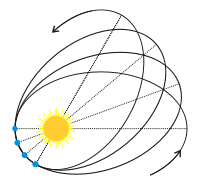
\includegraphics{figure/precessione_perielio}
  % figura presa da
  % http://commons.wikimedia.org/wiki/File:Perihelion_precession.svg
  \caption{Precessione del perielio di un pianeta}
  \label{fig:precessione-perielio}
\end{figure}
La prima legge di Keplero afferma che l'orbita descritta dai pianeti è
un'ellisse.  Questo risultato è rigorosamente vero nel caso in cui il pianeta
interagisce solo con la stella intorno a cui orbita.  La presenza di altri
eventuali pianeti perturba il sistema facendo in modo che l'orbita non sia
chiusa ma piuttosto una rosetta, si ha quindi una precessione del perielio, come
rappresentato nella figura~\ref{fig:precessione-perielio}.  Per esempio, dalle
osservazioni astronomiche si è scoperto che il perielio di Mercurio si sposta di
circa \ang{;;575} ogni cento anni.  Utilizzando la meccanica newtoniana e
tenendo conto della presenza di tutti i pianeti conosciuti si prevede una
precessione del perielio di Mercurio pari a circa \ang{;;532}.  Per spiegare
questa incongruenza sono state proposte diverse ipotesi, fra cui la presenza di
un corpo perturbante come un nuovo pianeta (Vulcano), più interno di Mercurio, o
un satellite di Mercurio.  Tuttavia questi corpi non sono mai stati trovati e
faremo vedere che la relatività generale è in grado di risolvere questo
problema.

% TODO: capire per bene i passaggi dell'Adler
Per determinare l'orbita di un pianeta abbiamo bisogno di quattro equazioni per
le quattro coordinate spazio-temporali sferiche $t$, $r$, $\theta$ e $\phi$.
Una prima equazione differenziale per la coordinata $r$ si ottiene dividendo
l'intervallo di tempo proprio di Schwarzschild~\eqref{eq:metrica-schwarzschild}
per $\dd\tau^{2}$
\begin{equation}
  \label{eq:mercurio-r}
  \bigg(\toder{\tau}{\tau}\bigg)^{2} = 1 = \bigg(1 -
  \frac{r_{\textup{S}}}{r}\bigg)\dot{t}^{2} - \bigg(1 -
  \frac{r_{\textup{S}}}{r}\bigg)^{-1}\dot{r}^{2} - r^{2}(\dot{\theta}^{2} +
  \sin^{2}\theta \dot{\phi}^{2}).
\end{equation}
Il punto sopra le variabili indica la derivazione rispetto al tempo proprio
$\tau$.  Per determinare le altre equazioni dobbiamo risolvere il problema
variazionale
\begin{equation}
  \delta \int \dd \tau = 0
\end{equation}
in cui $\dd\tau$ è la metrica di Schwarzschild.  Questo problema può essere
risolto più facilmente considerando la seguente formulazione equivalente
\begin{equation}
  \begin{split}
    \delta\int \dd\tau &= \delta \int \bigg(\toder{\tau}{\tau}\bigg)^{2} \dd
    \tau \\
    &= \delta \int \bigg(\bigg(1 - \frac{r_{\textup{S}}}{r}\bigg)\dot{t}^{2} -
    \bigg(1 - \frac{r_{\textup{S}}}{r}\bigg)^{-1}\dot{r}^{2} -
    r^{2}(\dot{\theta}^{2} + \sin^{2}\theta \dot{\phi}^{2}) \bigg) \dd \tau = 0.
  \end{split}
\end{equation}
Da qui, considerando la funzione integranda come una lagrangiana, si ottengono
tre equazioni di Eulero-Lagrange per le coordinate, rispettivamente, $\theta$,
$\phi$ e $t$
\begin{subequations}
  \begin{gather}
    \toder{}{\tau}(r^{2}\dot{\theta}) = r^{2}\sin\theta\cos\theta
    \dot{\phi}^{2}, \label{eq:mercurio-mu} \\
    \toder{}{\tau}(r^{2} \sin^{2}\theta \dot{\phi}) = 0, \label{eq:mercurio-phi}
    \\
    \toder{}{\tau}\bigg(\bigg(1 - \frac{r_{\textup{S}}}{r}\bigg) \dot{t} \bigg)
    = 0. \label{eq:mercurio-t}
  \end{gather}
\end{subequations}
Non abbiamo scritto l'equazione di Eulero-Lagrange per la coordinata $r$ poiché
utilizzeremo la~\eqref{eq:mercurio-r}.

Notiamo che associando all'equazione differenziale~\eqref{eq:mercurio-mu} le
condizioni iniziali $\theta = \pi/2$ e $\dot{\theta} = 0$, la funzione costante
$\theta(\tau) = \pi/2$ costituisce l'unica soluzione di questo problema di
Cauchy.  Ciò significa che con un'opportuna scelta delle coordinate il moto del
pianeta si svolge in un piano, così come succede anche in meccanica classica.
Sostituendo $\theta = \pi/2$ nella~\eqref{eq:mercurio-phi} abbiamo
\begin{equation}
  \label{eq:mercurio-phi2}
  \toder{}{\tau}(r^{2}\dot{\phi}) = 0 \implies r^{2}\dot{\phi} = h =
  \text{costante}
\end{equation}
cioè il pianeta si muove con velocità areolare costante, come nel problema di
Keplero classico.  Invece dalla~\eqref{eq:mercurio-t} otteniamo
\begin{equation}
  \label{eq:mercurio-t2}
  \bigg(1 - \frac{r_{\textup{S}}}{r}\bigg)\dot{t} = l = \text{costante}.
\end{equation}
Sostituendo tutti questi risultati nella~\eqref{eq:mercurio-r} troviamo
\begin{equation}
  \label{eq:mercurio-r2}
  1 = \bigg(1 - \frac{r_{\textup{S}}}{r}\bigg)^{-1}l^{2} - \bigg(1 -
  \frac{r_{\textup{S}}}{r}\bigg)^{-1}\dot{r}^{2} - \frac{h^{2}}{r^{2}}.
\end{equation}

Per determinare l'equazione dell'orbita conviene pensare la coordinata $r$ come
funzione di $\phi$, quindi indicando con l'apice la derivazione rispetto a
$\phi$ abbiamo
\begin{equation}
  \dot{r} = \toder{r}{\tau} = \toder{r}{\phi} \toder{\phi}{\tau} = r' \dot{\phi}
  = r' \frac{h}{r^{2}}
\end{equation}
e ponendo $u = 1/r$, con
\begin{equation}
  \dot{r} = \frac{h}{r^{2}}r' = \frac{h}{r^{2}}\toder{r}{\phi} =
  hu^{2}\toder{}{\phi} \frac{1}{u} = -hu^{2}\frac{u'}{u^{2}} = -hu',
\end{equation}
la~\eqref{eq:mercurio-r2} diventa
\begin{equation}
  1 - r_{\textup{S}}u = l^{2} - h^{2}u'^{2} - h^{2}u^{2}(1 - r_{\textup{S}}u),
\end{equation}
da cui, riarrangiando,
\begin{equation}
  \label{eq:mercurio-u'}
  u'^{2} = \frac{l^{2} - 1}{h^{2}} + \frac{r_{\textup{S}}}{h^{2}}u - u^{2} +
  r_{\textup{S}}u^{3} \equiv f(u).
\end{equation}
Questa equazione può essere integrata nel seguente modo
\begin{equation}
  \toder{u}{\phi} = \sqrt{f(u)} \implies \dd\phi = f^{-1/2}(u) \dd u \implies
  \phi = \phi_{0} + \int_{u_{0}}^{u} f^{-1/2}(\tilde{u}) \dd \tilde{u}.
\end{equation}
Sebbene questa sia una soluzione esatta, non è utile a livello pratico perché
fornisce solo un'espressione implicita di $u$, e quindi $r$, rispetto a $\phi$.
Nella risoluzione del problema di Keplero classico si giunge all'equazione di
Binet che è un'equazione differenziale del secondo ordine in $u$.  Per risolvere
il problema nella relatività generale, a questo punto, l'idea è quella di
ottenere un'equazione differenziale del secondo ordine in $u$ da confrontare con
l'equazione di Binet.  Derivando rispetto a $\phi$ la~\eqref{eq:mercurio-u'}
abbiamo
\begin{equation}
  \label{eq:mercurio1}
  2u'u'' = \frac{r_{\textup{S}}}{h^{2}}u' - 2uu' + 3r_{\textup{S}}u^{2}u'
  \implies u'\bigg(2u'' - \frac{r_{\textup{S}}}{h^{2}} + 2u -
  3r_{\textup{S}}u^{2}\bigg) = 0.
\end{equation}
Una soluzione di questa equazione è $u' = 0$, cioè
$u(\phi) = 1/r(\phi) = \text{costante}$.  Tuttavia questa situazione non ci
interessa poiché descrive un moto circolare, essendo la distanza dal centro del
campo costante, quindi non c'è un perielio e non è possibile osservare la sua
precessione.  L'altra possibile soluzione è
\begin{equation}
  \label{eq:binet-relativ}
  2u'' - \frac{r_{\textup{S}}}{h^{2}} + 2u - 3r_{\textup{S}}u^{2} = 0 \implies
  u'' + u = \frac{r_{\textup{S}}}{2h^{2}} + \frac{3}{2}r_{\textup{S}}u^{2} =
  \frac{GM}{r^{4}(\ltoder{\phi}{\tau})^{2}} + \frac{3}{2}r_{\textup{S}}u^{2},
\end{equation}
in cui $M$ è la massa del corpo che genera il campo gravitazionale.  Nel
problema di Keplero classico, l'\index{equazione!di Binet}equazione di Binet è
\begin{equation}
  \label{eq:binet}
  u'' + u = \frac{GM}{r^{4}(\ltoder{\phi}{t})^{2}}.
\end{equation}
Osserviamo che per piccole velocità
$\ltoder{\phi}{\tau} \approx \ltoder{\phi}{t}$.  Inoltre per i pianeti del
sistema solare risulta
\begin{equation}
  \frac{3r_{\textup{S}}u^{2}/2}{r_{\textup{S}}/(2h^{2})} = 3u^{2}h^{2} \ll 1,
\end{equation}
infatti
\begin{equation}
  3u^{2}h^{2} = \frac{3}{r^{2}}r^{4} \bigg(\toder{\phi}{\tau}\bigg)^{2} = 3r^{2}
  \bigg(\toder{\phi}{\tau}\bigg)^{2} \approx 3 v_{\textup{t}}^{2},
\end{equation}
in cui $v_{\textup{t}} = r\ltoder{\phi}{t}$ è la velocità tangenziale del corpo,
espressa in unità di $c$ poiché abbiamo posto $c = 1$.  Per Mercurio, il pianeta
più interno del sistema solare e quindi con la maggior velocità tangenziale,
$3 v_{\textup{t}}^{2} = \num{7.7e-8}$, quindi possiamo considerare il termine
$3r_{\textup{S}}u^{2}/2$ nella~\eqref{eq:binet-relativ} come una debole
perturbazione.  In dettaglio, vogliamo risolvere l'equazione
\begin{equation}
  u'' + u = A + \frac{\epsilon u^{2}}{A},
\end{equation}
con $A = r_{\textup{S}}/(2h^{2})$ e $\epsilon = 3Ar_{\textup{S}}/2  \ll 1$.
Cerchiamo soluzioni del tipo
\begin{equation}
  u(\phi) = u_{0}(\phi) + \epsilon v(\phi),
\end{equation}
con $u_{0}(\phi)$ soluzione dell'equazione di Binet classica
\begin{equation}
  \label{eq:binet-2}
  u_{0}'' + u_{0} = A
\end{equation}
cioè
\begin{equation}
  u_{0} = A + B\cos(\phi + \phi_{0}),
\end{equation}
con $B$ e $\phi_{0}$ costanti reali di integrazione.  Ruotando opportunamente il
sistema di riferimento si può fare in modo che $\phi_{0} = 0$ cosicché $u_{0}$
diventa
\begin{equation}
  \label{eq:sol-binet}
  u_{0}(\phi) = A + B\cos\phi.
\end{equation}
Dunque l'equazione da risolvere è
\begin{equation}
  (u_{0}'' + \epsilon v'') + (u_{0} + \epsilon v) = A + \epsilon \frac{(u_{0} +
    \epsilon v)^{2}}{A} = A + \epsilon \frac{u_{0}^{2}}{A} +
  \mathcal{O}(\epsilon^{2}).
\end{equation}
Tenendo conto della~\eqref{eq:binet-2} l'equazione per $v(\phi)$ al primo ordine
in $\epsilon$ è
\begin{equation}
  \begin{split}
    v'' + v &= \frac{u_{0}^{2}}{A} = A + 2B\cos\phi +
    \frac{B^{2}}{A}\cos^{2}\phi \\
    &= \bigg(A + \frac{B^{2}}{2A}\bigg) + 2B\cos\phi +
    \frac{B^{2}}{2A}\cos(2\phi),
\end{split}
\end{equation}
in cui abbiamo ricordato l'identità trigonometrica
$\cos^{2}\phi = (1 + \cos(2\phi))/2$.  Dunque questa è l'equazione differenziale
del secondo ordine relativa al termine che perturba l'orbita dei pianeti.
Questa equazione è lineare, quindi la soluzione può essere espressa come somma
delle soluzioni delle tre equazioni seguenti
\begin{subequations}
  \begin{align}
    v_{a}'' + v_{a} &= A + \frac{B^{2}}{2A} \implies v_{a}(\phi) = A +
    \frac{B^{2}}{2A}, \\
    v_{b}'' + v_{b} &= 2B\cos\phi \implies v_{b}(\phi) = B\phi \sin\phi, \\
    v_{c}'' + v_{c} &= \frac{B^{2}}{2A}\cos(2\phi) \implies v_{c}(\phi) =
    -\frac{B^{2}}{6A}\cos(2\phi),
  \end{align}
\end{subequations}
dunque
\begin{equation}
  v(\phi) = v_{a}(\phi) + v_{b}(\phi) + v_{c}(\phi) = A + \frac{B^{2}}{2A} +
  B\phi\sin\phi - \frac{B^{2}}{6A}\cos(2\phi)
\end{equation}
e in questo modo $u(\phi)$ è data da
\begin{equation}
  \begin{split}
    u(\phi) &= u_{0}(\phi) + \epsilon v(\phi) \\
    &= A + B\cos\phi + \epsilon A + \frac{\epsilon B^{2}}{2A} + \epsilon
    B\phi\sin\phi - \frac{\epsilon B^{2}}{6A}\cos(2\phi).
  \end{split}
\end{equation}
Al primo ordine in $\epsilon$ abbiamo
\begin{equation}
  \cos(\phi - \epsilon\phi) = \cos\phi \cos(\epsilon\phi) + \sin\phi
  \sin(\epsilon\phi) \approx \cos\phi + \epsilon\phi\sin\phi,
\end{equation}
allora
\begin{equation}
  \frac{1}{r(\phi)} = u(\phi) \approx A + B\cos(\phi - \epsilon\phi) +
  \epsilon\bigg(A + \frac{B^{2}}{2A} - \frac{B^{2}}{6A}\cos(2\phi)\bigg).
\end{equation}
L'ultimo termine, fra parentesi, induce una piccola variazione nella distanza
radiale del pianeta, ma non può essere responsabile della precessione del
perielio poiché il termine $\cos(2\phi)$ ha periodo sottomultiplo intero di
$2\pi$ (quindi dopo un'intera rivoluzione di $\var \phi = 2\pi$ assume di nuovo
lo stesso valore).  Il resto della funzione $u(\phi)$ si differenzia dalla
soluzione~\eqref{eq:sol-binet} dell'equazione di Binet per la presenza di
$-\epsilon\phi$ nell'argomento del coseno.  Il perielio si ha quando $r(\phi)$ è
minimo, vale a dire quando $u(\phi)$ è massimo e ciò si verifica quando il
coseno del secondo termine vale $1$, cioè quando
\begin{equation}
  \phi_{n}(1 - \epsilon) = 2\pi n \implies \phi_{n} = \frac{2\pi n}{1 -
    \epsilon} \approx 2\pi n(1 + \epsilon)
\end{equation}
con $n$ numero di rivoluzioni compiute dal pianeta intorno al Sole a partire da
un istante iniziale fissato.  Il perielio successivo si ha dopo una variazione
della coordinata $\phi$ di
\begin{equation}
  \var\phi = \phi_{n+1} - \phi_{n} = 2\pi(1 + \epsilon)
\end{equation}
invece di $2\pi$ come succede per un'orbita chiusa.  La relatività generale
prevede allora una precessione del perielio dei pianeti nel loro moto intorno al
Sole, indipendentemente dalla presenza perturbatrice di altri corpi.  Stimiamo
il valore $\delta\phi$ di questa precessione per verificare se è in accordo con
i dati sperimentali.  Per i pianeti del sistema solare
$r_{\textup{S}} = 2GM_{\odot}$ è il raggio di Schwarzschild del Sole, allora
\begin{equation}
  \delta\phi = 2\pi\epsilon = 2\pi \frac{3}{4}\frac{r_{\textup{S}}^{2}}{h^{2}} =
  6\pi \frac{G^{2}M_{\odot}^{2}}{h^{2}}.
\end{equation}
In particolare per il pianeta Mercurio si ha
\begin{equation}
  \delta\phi = \ang{;;0.1036}
\end{equation}
e la precessione dopo cento anni, ricordando che il suo periodo orbitale è di
$87.8$ giorni, è data da
\begin{equation}
  \delta_{100}\phi = \frac{\delta\phi \cdot 100 \cdot 365.25}{87.8} =
  \ang{;;43}.
\end{equation}
All'inizio della sezione abbiamo ricordato che la precessione secolare di
Mercurio è di circa \ang{;;575}, possiamo ora concludere che di questi, circa
\ang{;;43} sono dovuti a effetti di relatività generale e circa \ang{;;532} alla
perturbazione indotta dalla presenza degli altri pianeti.  Mercurio è il pianeta
del sistema solare per il quale la precessione relativistica del perielio è più
evidente in quanto è il più interno e quindi il più influenzato dal campo
gravitazionale del Sole.

\subsection{Deflessione della luce}
\label{sec:deflessione-luce}

Secondo la teoria newtoniana, solo i corpi dotati di massa sono soggetti
all'attrazione gravitazionale.  In questo paragrafo vedremo che un fotone (così
come qualsiasi corpo privo di massa) risente della presenza di un campo
gravitazionale, come quello generato dal Sole, deviando la propria traiettoria.
Questo fenomeno è comprensibile ricordando che tutti i corpi si muovono lungo
geodetiche in uno spazio-tempo curvo.

% TODO: non ho mai classificato gli intervalli nei tipi `luce', `spazio' o
% `tempo', quindi o lo faccio da qualche parte o riformulo la frase seguente.
% Dovrei anche spiegare cos'è la linea d'universo.
In relatività speciale, per due eventi separati da un intervallo di tipo luce la
distanza vale $\dd\tau^{2} = 0$ e assumiamo che lo stesso valga anche in
relatività generale.  Assumiamo inoltre che l'equazione della
geodetica~\eqref{eq:geodetica} sia valida anche per le particelle prive di massa
come i fotoni.  Tuttavia dobbiamo fare attenzione al fatto che, proprio in virtù
del fatto che $\dd\tau^{2} = 0$, non possiamo parametrizzare la linea d'universo
di un fotone, o di una qualsiasi particella con massa nulla, usando il tempo
proprio $\tau$.  Piuttosto dobbiamo utilizzare un differente parametro $q$ tale
che l'equazione della geodetica
\begin{equation}
  \toder[2]{x^{\mu}}{q} + \tensor{\Gamma}{^{\mu}_{\lambda\nu}}
  \toder{x^{\lambda}}{q} \toder{x^{\nu}}{q} = 0
\end{equation}
abbia senso.  A partire da questa equazione si possono ricavare nuovamente,
sempre con l'assunzione $\theta = \pi/2$, le relazioni~\eqref{eq:mercurio-phi2}
e \eqref{eq:mercurio-t2}.  La~\eqref{eq:mercurio-r2} va modificata in questo
modo tenendo conto del fatto che $\dd\tau^{2} = 0$
\begin{equation}
  0 = \bigg(1 - \frac{r_{\textup{S}}}{r}\bigg)^{-1}l^{2} - \bigg(1 -
  \frac{r_{\textup{S}}}{r}\bigg)^{-1}\dot{r}^{2} - \frac{h^{2}}{r^{2}}.
\end{equation}
Svolgendo i calcoli in maniera analoga a quanto visto nel paragrafo precedente e
ponendo sempre $u = 1/r$ si arriva all'equazione
\begin{equation}
  u'\bigg(u'' + u - \frac{3}{2}r_{\textup{S}}u^{2}\bigg) = 0.
\end{equation}
Si possono avere due situazioni:
\begin{equation}
  \label{eq:deflessione1}
  u'' + u - \frac{3}{2}r_{\textup{S}}u^{2} = 0,
\end{equation}
oppure
\begin{equation}
  u' = 0 \implies u(\phi) = u_{0} = \text{costante},
\end{equation}
ma quest'ultima soluzione deve essere scartata per ragioni di stabilità.
Osserviamo che si poteva giungere direttamente alla~\eqref{eq:deflessione1}
partendo dalla~\eqref{eq:mercurio1} e ponendo
$\dd\tau^{2} = 0 \implies 1/h^{2} = (\ltoder{\tau}{\phi})^{2}/r^{4} = 0$.  Il
termine $3r_{\textup{S}}u^{2}/2$ è una piccola perturbazione rispetto a $u$,
infatti
\begin{equation}
  \frac{3r_{\textup{S}}u^{2}/2}{u} = \frac{3r_{\textup{S}}u}{2} =
  \frac{3r_{\textup{S}}}{2r}.
\end{equation}
Considerando il caso del Sole, $r_{\textup{S}} = \SI{3}{\kilo\metre}$ e la
distanza $r$ rispetto alla sua origine a cui un fotone può passare è maggiore o
uguale al raggio $R_{\odot} = \SI{7e5}{\kilo\metre}$, quindi
$3r_{\textup{S}}u^{2}/(2u) \ll 1$.  Allora cerchiamo una soluzione dell'equazione
\begin{equation}
  u'' + u = \epsilon u^{2},
\end{equation}
con $\epsilon = 3r_{\textup{S}}/2$, del tipo
\begin{equation}
  u(\phi) = u_{0}(\phi) + \epsilon v(\phi).
\end{equation}
Sostituendo nell'equazione da risolvere abbiamo
\begin{equation}
  \label{eq:deflessione2}
  u_{0}'' + u_{0} + \epsilon v'' + \epsilon v = \epsilon u_{0}^{2} +
  \mathcal{O}(\epsilon^{2}).
\end{equation}
I termini di ordine zero in $\epsilon$ danno
\begin{equation}
  u_{0}'' + u_{0} = 0,
\end{equation}
la cui soluzione generale è
\begin{equation}
  u_{0}(\phi) = A\cos(\phi + \phi_{0}),
\end{equation}
con $A$ e $\phi_{0}$ costanti di integrazione.  Ruotando il sistema di
coordinate è possibile annullare $\phi_{0}$ cosicché il valore approssimato
$r = 1/u_{0}$ della coordinata radiale soddisfi la relazione
\begin{equation}
  r \cos\phi = \frac{1}{A} = \text{costante}.
\end{equation}
Il prodotto $r\cos\phi$ è la coordinata cartesiana $x$, quindi questa è
l'equazione di una retta parallela all'asse $y$.  Potevamo attenderci questo
risultato: in prima approssimazione il raggio di luce non viene deviato dal
campo gravitazionale del Sole.  Inoltre la distanza $r_{0}$ di minimo
avvicinamento al corpo si ha per $\cos\phi = 1$, cioè
$r_{0} = 1/A \implies u_{0} = (\cos\phi)/r_{0}$.  Uguagliando i termini di
ordine uno in $\epsilon$ troviamo
\begin{equation}
  \label{eq:deflessione3}
  v'' + v = u_{0}^{2} = \frac{\cos^{2}\phi}{r_{0}^{2}} = \frac{1 +
    \cos(2\phi)}{2r_{0}^{2}}.
\end{equation}
Cerchiamo soluzioni del tipo
\begin{equation}
  v(\phi) = \alpha + \beta\cos(2\phi)
\end{equation}
con $\alpha$ e $\beta$ costanti di integrazione da determinare.  Sostituendo
nella~\eqref{eq:deflessione3} otteniamo
\begin{equation}
  v'' + v = \alpha - 3\beta\cos(2\phi).
\end{equation}
Confrontando con la~\eqref{eq:deflessione3} abbiamo
\begin{subequations}
  \begin{align}
    \alpha &= \frac{1}{2r_{0}^{2}}, \\
    \beta &= - \frac{1}{6r_{0}^{2}},
  \end{align}
\end{subequations}
quindi
\begin{equation}
  v(\phi) = \frac{1}{2r_{0}^{2}} - \frac{\cos(2\phi)}{6r_{0}^{2}} =
  \frac{2}{3r_{0}^{2}} - \frac{\cos^{2}\phi}{3r_{0}^{2}}.
\end{equation}
In definitiva
\begin{equation}
  \label{eq:deflessione4}
  u(\phi) = u_{0}(\phi) + \epsilon v(\phi) = \frac{\cos\phi}{r_{0}} +
  \frac{2\epsilon}{3r_{0}^{2}} - \frac{\epsilon\cos^{2}\phi}{3r_{0}^{2}}.
\end{equation}
% TODO: fare una figura altrimenti si capisce piuttosto poco e riformulare il
% testo seguente in modo da adattarsi alla figura.
La traiettoria del fotone è, dunque, una retta (data dal termine
$(\cos\phi)/r_{0}$) disturbata da una piccola perturbazione dell'ordine di
$\epsilon$.  L'effetto di questa perturbazione è il seguente: il fotone si
avvicina al Sole in linea retta, quando l'influenza del campo gravitazionale
della stella non è più trascurabile il fotone viene leggermente deflesso, quindi
si allontana nuovamente in linea retta.  Calcoliamo la deflessione del fotone.
Le direzioni asintotiche seguite dal fotone si ottengono calcolando il limite
$r \to \infty$ o, il che è equivalente, $u \to 0$ nella~\eqref{eq:deflessione4}
\begin{equation}
  0 = \frac{\cos\phi}{r_{0}} + \frac{2\epsilon}{3r_{0}^{2}} -
  \frac{\epsilon\cos^{2}\phi}{3r_{0}^{2}} \implies \cos^{2}\phi -
  \frac{3r_{0}}{\epsilon}\cos\phi - 2 = 0.
\end{equation}
Le soluzioni sono
\begin{equation}
  \cos\phi = \frac{3r_{0}}{2\epsilon}\bigg(1 \pm \sqrt{1 +
    \frac{8\epsilon^{2}}{9r_{0}^{2}}}\bigg),
\end{equation}
ma l'unica accettabile è quella con il segno $-$, poiché quella con il segno $+$
rende il coseno maggiore di $1$.  Sviluppando la soluzione accettabile al primo
ordine in $\epsilon$ abbiamo
\begin{equation}
  \cos\phi = \frac{3r_{0}}{2\epsilon}\bigg(1 - \sqrt{1 +
    \frac{8\epsilon^{2}}{9r_{0}^{2}}}\bigg) \approx \frac{3r_{0}}{2\epsilon}\bigg(1 - 1 -
  \frac{4\epsilon^{2}}{9r_{0}^{2}}\bigg) = -\frac{2\epsilon}{3r_{0}} =
  -\frac{r_{\textup{S}}}{r_{0}}.
\end{equation}
Abbiamo già osservato che per i fotoni che passano nelle vicinanze del Sole
risulta $r_{\textup{S}}/r \ll 1$, quindi $\phi \approx \pm \pi/2$, allora
possiamo porre $\phi = \pi/2 + \delta$, con $\delta \ll 1$, da cui
\begin{equation}
  -\frac{r_{\textup{S}}}{r_{0}} = \cos\phi = \cos(\pi/2 + \delta) = -\sin\delta.
\end{equation}
Dal momento che $\delta$ è molto piccolo possiamo approssimare il seno
dell'angolo con l'angolo stesso e quindi
\begin{equation}
  \delta = \frac{r_{\textup{S}}}{r_{0}}.
\end{equation}
La deflessione $\var$ è il doppio di questo angolo, dunque, ripristinando il
valore della velocità della luce,
\begin{equation}
  \var = 2\delta = \frac{2r_{\textup{S}}}{r_{0}} = \frac{4GM}{c^{2}r_{0}}.
\end{equation}

Per quanto riguarda la deviazione dei raggi di luce da parte del campo
gravitazionale del Sole, supponendo che la distanza di minimo avvicinamento sia
proprio pari al raggio solare $R_{\odot}$, l'angolo di deflessione vale
\begin{equation}
  \var_{\odot} = \frac{4GM_{\odot}}{c^{2}R_{\odot}} = \ang{;;1.75}.
\end{equation}
Questa previsione teorica è stata confermata in numerosi esperimenti via via più
accurati, il primo dei quali fu realizzato da Eddington durante l'eclissi totale
di Sole del 1919.

\subsection{Ritardo dei segnali radar}
\label{sec:ritardo-radar}

L'ultimo fenomeno di cui ci interessiamo è il ritardo nel tempo di volo dei
segnali radar rispetto a quanto previsto dalla relatività speciale in uno
spazio-tempo piatto.  Ciò è dovuto al fatto che i fotoni non si muovono lungo
linee rette ma lungo le geodetiche, che hanno lunghezza maggiore rispetto alle
linee rette in uno spazio-tempo piatto.  Questo fenomeno può essere osservato
inviando un segnale radar a un pianeta in congiunzione superiore e misurando il
tempo necessario affinché il segnale vada verso il pianeta e torni sulla Terra.
Tuttavia l'esecuzione di esperimenti su questo fenomeno presentano delle
difficoltà di tipo pratico, delle quali non ci occuperemo.

% TODO: mettere anche qui una figura e rielaborare il testo altrimenti non si
% capisce niente.  Dopo aver fatto la figura, parlare in generale di distanza di
% minimo avvicinamento piuttosto che di raggio solare.
Senza entrare nei dettagli dei conti forniamo i risultati delle previsioni
teoriche della relatività
generale.\footnote{Questo problema è trattato da
  \textcite[1103-1109]{misner:gravitation},
  \textcite[201-207]{weinberg:gravitation}.}
In un spazio-tempo piatto, il tempo $\tau(r,R_{\odot})$ necessario per un fotone
per giungere tangente sulla superficie del Sole da un punto a distanza $r$ dal
centro della stella è dato semplicemente dal rapporto fra la distanza euclidea
fra questi due punti e la velocità dei fotoni nel vuoto
\begin{equation}
  \tau(r, R_{\odot}) = \frac{\sqrt{r^{2} - R_{\odot}^{2}}}{c}.
\end{equation}
La correzione relativistica per $\tau(r, R_{\odot})$, che tiene conto della
curvatura dello spazio tempo prodotta dal campo gravitazionale del Sole, è
\begin{equation}
  \begin{split}
    t(r,R_{\odot}) &\approx \tau(r,R_{\odot}) + \var t(r,R_{\odot}) \\
    &= \frac{\sqrt{r^{2} - R_{\odot}^{2}}}{c} + \frac{2GM_{\odot}}{c^{3}} \ln
    \frac{r + \sqrt{r^{2} - R_{\odot}^{2}}}{R_{\odot}} +
    \frac{GM_{\odot}}{c^{3}} \sqrt{\frac{r - R_{\odot}}{r + R_{\odot}}}.
  \end{split}
\end{equation}
Il tempo $t_{\textup{tot}}$ totale di volo del fotone per andare dalla Terra, a
distanza $r_{1}$ dal Sole, a un pianeta a distanza $r_{2}$ in congiunzione
superiore è
\begin{equation}
  \begin{split}
    t_{\textup{tot}} &= 2(t(r_{1},R_{\odot}) + t(r_{2},R_{\odot})) \\
    &= 2(\tau(r_{1},R_{\odot}) + \var t(r_{1},R_{\odot}) +
    \tau(r_{2},R_{\odot}) + \var t(r_{2},R_{\odot})).
  \end{split}
\end{equation}
Considerando il sistema Terra-Mercurio, il ritardo
$\var t = 2(\var t(r_{1},R_{\odot}) + \var t(r_{2},R_{\odot}))$ rispetto alla
previsione $2(\tau(r_{1},R_{\odot}) + \tau(r_{2},R_{\odot}))$ in uno
spazio-tempo piatto vale \SI{240}{\micro\second}, che corrisponde a una distanza
di \SI{72}{\kilo\metre}, su un tempo di volo totale $t_{\textup{tot}}$ di
\SI{20}{\minute}.

%%% Local Variables:
%%% mode: latex
%%% TeX-master: "../gravitazione"
%%% fill-column: 80
%%% End:
